%!TEX root = ../../prace.tex


\section{Stávající implementace mechanismů}

Rozebereme si, jakým způsobem je v současné době přistupováno k blokům a jak jsou tyto bloky umisťovány do herního světa. Dále nás budou zajímat ostatní herní mechaniky, jako například denní cyklus, nebo jakým způsobem je řešena herní postava, její inventář a možnosti hráče interakce se světem. Poté se rozhodneme, jakým způsobem budeme uvedené mechaniky řešit my.

\subsection{Bloky}
\label{subsec:blocks}

Pod pojmem \uv{blok} budeme chápat objekt, který je umístěn v~nějaké ortogonální mřížce 3D prostoru a~beze zbytku tento prostor vyplňuje. Bloky spolu sdílí společnou množinu vlastností a dále pak samy definují své vlastní vlastnosti, které vychází z povahy bloku, tedy toho, co daný blok reprezentuje. V této kapitole rozebereme tyto vlastnosti a následně definujeme, jaké problémy budeme muset v této práci řešit.


\subsubsection{Základní vlastnosti}

Mezi základní vlastnosti bloku bychom měli zařadit \textit{vizuální reprezentaci}, \textit{pozici ve světě}, \textit{rotaci} a \textit{velikost}. Tento výčet není kompletní, ale můžeme říct, že jsou pro hráče nejvíce viditelné. Podle typu hry, jejího stylu a celkové koncepce bychom pak mohli do této množiny přidat třeba \textit{zdraví bloku}. V této části se zaměříme právě na základní vlastnosti a rozšiřujícím vlastnostem se budeme věnovat v následujících částech této kapitoly.

Vizuální reprezentace zřejmě vychází z povahy bloku. Vždy ale platí, že se vždy musí vejít do nějakých hranic bloku, obvykle daných v rámci pravidelné mřížky, ve které se blok nachází. Může v sobě zahrnovat i nějaké informace, které jsou pak hráčem vnímány pohledem. Kupříkladu mohou různými způsoby indikovat vnitřní stav objektu, podobně jako třeba svítivé diody indikují různé stavy elektronických zařízení v reálném světě. Podrobněji se budeme vzhledem zabývat až budeme řešit konkrétní bloky v naší hře.

Pozice bloku v herním světě je u her z kapitoly \ref{chap:uvod} může být buď na jednoznačně definovaném místě v herním světě, přičemž všechny bloky mají vůči sobě stejnou rotaci (\MC{}), nebo je blok součástí nějaké skupiny\footnote{Za skupinu budeme považovat shluk alespoň jednoho bloku a všechny bloky ve skupině musí být ve stejné mřížce.} bloků s jednoznačnou pozicí v herním světě. Tato skupina pak může mít libovolnou rotaci vůči nějakému globálnímu souřadnicovému systému a můžeme říct, že tato skupina tvoří lokální ortogonální systém. Různé skupiny mohou být vůči sobě různě natočeny. Toto chování je možné pozorovat třeba ve hře \ME{}, kde postavením prvního bloku určíme pozici a rotaci této skupiny. Pokud budeme chtít přidat do světa další blok, do nějaké vzdálenosti od prvního bloku je tento nově stavěný blok stále přichytáván do mřížky definované prvním blokem a rotace bloku jsou vždy o 90~stupňů. Obvykle platí, že první blok je umístěn vodorovně (tedy krychle bude i na šikmém terénu umístěna tak, že její horní a dolní strana je ve vodorovné poloze) a je možné ho libovolně rotovat kolem vertikální osy.

Rotace bloků jsou u naprosté většiny her řešeny v zásadě podobně. Výjimkou je pouze \MC{}, který rotaci bloků neumožňuje. U většiny bloků to nevadí, protože jsou bloky umístěny po směru, ze kterého je blok umisťován. Můžeme však nalézt některé speciality, třeba blok \textit{kolejí} (oficiální popis bloku \citep{mc_rail}). Koleje v \MC{u} mohou být rovné (ve směru sever -- jih nebo východ -- západ), mohou být nakloněné a překonávat výškový rozdíl mezi dvěma bloky, nebo mohou tvořit zatáčku. Díky absenci rotací tak hra používá několik pravidel, které určují výslednou podobu bloku. Podrobněji se jimi však zabývat nemusíme. U zbývajících her je situace, kterou jsme popsali v úvodu této části -- první blok je natočen vodorovně, má libovolnou rotaci dle vertikální osy a tímto určuje přichytávací mřížku pro další stavěné bloky.

Hry mají velikost bloků vždy stejně velkou. \MC{} má hranu bloku o~délce $1\,\rm m$ (popis bloku na oficiální Wiki stránce Minecraftu \citep{mc_block}, oficiální popis jednotek použitých v Minecraftu \citep{mc_units}). \SE{} sice bloky hranově omezuje dle kategorií od $0,5\,\rm m$ do $2,5\,\rm m$ (oficiální popis bloků ve hře \citep{se_blocks_wiki}), ale tyto kategorie mezi sebou nelze kombinovat a je možné k sobě vázat pouze bloky z jedné a té samé kategorie. U ostatních her je situace podobná, byť některé jsou v raných fázích vývoje a tudíž pro ně neexistuje žádný oficiální zdroj informací, takže velikosti bloků bychom mohli pouze odhadovat. 

Jako další základní vlastnosti bloku bychom mohli brát třeba \textit{zdraví}, \textit{cenu za postavení}, \textit{čas doby stavby}, \textit{délku trvání destrukce} (pokud vychází z hráčovy akce), co hráč získá za zničení bloku apod. U doby konstrukce a destrukce bloku můžeme říct, že doba trvání dané akce závisí na parametrech bloku a použitém nástroji. Kupříkladu v \MC{u} trvá kutání bloku kamene \textit{diamantovým} krumpáčem podstatně rychleji, než při použití krumpáče \textit{dřevěného}. Taktéž rychlost opotřebení nástrojů je různá. Nicméně když se ve hrách přepneme do tzv.~\textit{kreativního} módu, pak máme stavbu bloků \uv{zadarmo} a ihned. Tedy nemusíme mít žádné komponenty ke stavbě, ani specializovaný nástroj (případ \SE{}, \ME{}), nebo nám při postavení bloku tyto bloky neubývají z inventáře (\MC{}). 

\subsubsection{Součásti bloků}
Jako součásti bloků můžeme brát cokoliv, co rozšiřuje základní vlastnosti. Zde bychom mohli zmínit třeba \textit{Redstone} v \MC{u}. Redstone je speciální typ bloku, chová se jako elektrický vodič a v kombinaci s jinými bloky je možné vytvářet logická hradla. Je zřejmé, že pokud vhodným způsobem zkombinujeme určitá hradla, je možné v \MC{u} vytvořit třeba bitovou sčítačku. Ačkoliv vytvoření jednoho hradla je snadné, složitější logické obvody (například kódový zámek) jsou pak velmi náročné na prostor. Nejen z tohoto důvodu pro \MC{} vnikly různé módy, rozšiřující základní funkcionalitu hry o nové elektrické komponenty. Pro zajímavost, mód \textit{RedPower} (blog autora \citep{eloraam}) má jednotlivá hradla jako samostatné bloky (což šetří místo) a navíc má možnost skládat různě barevné vodiče (což jsou pouze ekvivalenty Redstonových bloků) do sebe (až 16~linek signálu). Bez tohoto módu by hráč potřeboval takový prostor, aby položil 16~vedení Redstone tak, aby se nedotýkaly a vzájemně neovlivňovaly (na rovině by tyto vodiče zabíraly šířku 31~bloků). 

Další možné součásti bloků, kromě vedení elektřiny, může být například práce s kyslíkem či práce s inventářem. Některé bloky hráči nabízí nějaký úložný prostor, kam může přesunovat objekty ze svého inventáře. Později pak hráč může k bloku přijít a objekty si opět navrátit do svého inventáře. Zajímavou specialitou je náhled inventáře. Kupříkladu u hry \ME{} se jedná stůl a~jídlo na stole. Stůl má svůj inventář, do kterého je možné umisťovat jídlo. Ve hře je pak obsah inventáře stolu zobrazen tak, že jídlo má svůj náhledový model na talířích na stole, takže to vypadá, jako by bylo jídlo připraveno ke konzumaci. 


Dále můžeme zmínit interakci s uživatelem, ať už přímou, nebo nepřímou. Jako přímou interakci budeme chápat takové použití bloku, kdy rovnou vidíme nějakou změnu. To může být například stisknutí tlačítka, nebo změna polohy nějaké páky. Výsledek této přímé interakce pak hráč vidí okamžitě a vizuálně se blok nějakým způsobem změní. Jako nepřímou interakci bychom mohli uvést například otevření nějakého ovládacího rozhraní bloku, což je obvykle nějaká UI obrazovka. Obě interakce se mohou prolínat, takže výsledkem nepřímé interakce může být třeba změna barvy bloku.


\subsection{Komunikace bloků}
Bloky spolu mnohdy umí komunikovat. Dříve zmíněný Redstone z \MC{u} by se dal taktéž považovat za jistou metodu komunikace mezi bloky. Například stiskem tlačítka lze změnit výstupní Redstonový signál z tohoto tlačítka (třeba z neaktivního na aktivní), který způsobí změnu polohy nějakého pístu. Ovšem komunikace může být i méně viditelná -- například z terminálu v \SE{} je možné ovládat písty, otevírat a zavírat dveře hangáru apod. bez explicitních vodičů signálu.

Ve hrách \MC{} a \SE{} můžeme nalézt příklad dopravníkových systémů. Ty umožňují \uv{poslat} bloky či objekty na jiné místo, kupříkladu z jednoho křídla budovy do druhého. V \MC{u} bez módů se této funkcionality dá vcelku snadno dosáhnout, nicméně je to zdlouhavé a rychlost přesunu bloků je poměrně pomalá. Ale opět se můžeme obrátit na módy, třeba na \textit{BuildCraft} (oficiální stránky projektu \citep{buildcraft}), který umožňuje rychle dopravovat bloky i na velké vzdálenosti. Hra \SE{} má kvalitní dopravníkový systém už ve svém základu a slouží například pro dopravu natěženého materiálu od bloku \textit{Vrtáku} do bloku \textit{Skladiště} (který má svůj inventář). Svým způsobem je pak přeprava v rámci těchto systémů také druhem meziblokové komunikace - bloky si mezi sebou předávají konkrétní instance objektů.

\subsection{Skládání bloků do struktur}
Asi jediné příklady, který můžeme zmínit, jsou ve hře \MC{} -- postavení portálu do Netheru (obrázek \ref{fig:structs_nether_portal}), sněhuláka či golema. V momentě, kdy nějaká skupina bloků splňuje přesně definovaný tvar, tak se tyto bloky chápou jako jedna struktura a tak se s nimi i zachází. Portál je možné pomocí \textit{křesadla} aktivovat, ale pokud je portál aktivní a hráč odebere z portálu některý blok, který jej tvoří, portál se uzavře. Bloky ve tvaru sněhuláka a golema se po dokončení tvaru odeberou a namísto nich je do světa umístěno \NPC{} sněhuláka či golema.

\begin{figure}[!ht]\centering
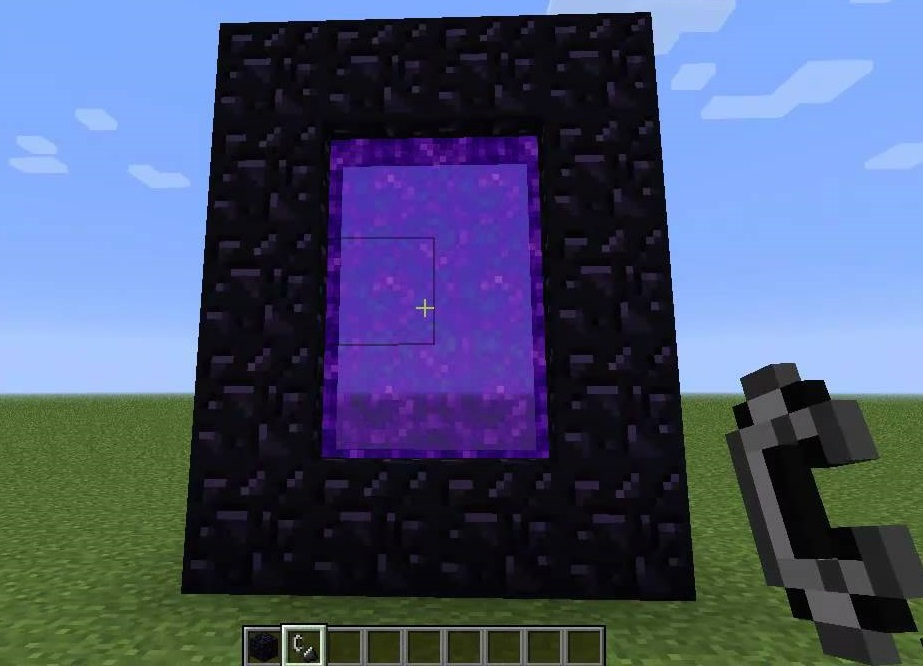
\includegraphics[ width=140mm]{../img/analysis/mc_portal}

\caption{Portál do Netheru. Zdroj: minecraftpocketedition.wikia.com \citep{mc_nether_portal}}
\label{fig:structs_nether_portal}

\end{figure}

\FloatBarrier



\subsubsection{Speciality}
Ve hrách \ME{} a  \NMS{} můžeme nalézt zajímavou funkcionalitu \textit{multibloků}. Tato funkcionalita nabízí například nahrazení nějaké stěny nějakého bloku oknem či nějakým dalším vizuálním či funkčním elementem.


Také bychom měli zmínit propagaci kyslíku v rámci postavených budov, kterou můžeme nalézt ve hrách \SE{} nebo \TM{}. Ačkoliv tento koncept je spíše vlastností herního prostředí, velice úzce souvisí s bloky. Pokud bloky tvoří uzavřenou strukturu, tak je možné vnitřní prostory natlakovat, zaplnit kyslíkem a sundat si helmu či dokonce celý skafandr. \SE{} využívá systém tzv.~\uv{místností} (oficiální dokumentace o kyslíku \citep{se_oxygen}). Místnosti lze zaplnit kyslíkem díky \textit{ventilaci}, což je blok, který umí do prostoru místnosti vhánět kyslík a také ho z něj odebírat. \TM{} dělá prakticky to samé, liší se pouze způsobem implementace rozpoznání místnosti, což souvisí se způsobem stavby bloků (jak jsme zmínili v kapitole \ref{chap:uvod}).


\subsection{Herní svět}

V této části se zaměříme na zpracování herního světa a s tím souvisejících mechanik.

\subsubsection{Reprezentace}

Pokud shrneme poznatky z kapitoly \ref{chap:uvod}, tak můžeme říct, že máme v zásadě dvě možnosti. Buď můžeme po vzoru \MC{} mít celý svět tvořen bloky. Pak bychom kvůli optimalizaci výkonu také museli tyto bloky shlukovat do skupin (v \MC{u} se jim říká \textit{chunks} a jsou velké $16*16*256$ bloků). Nebo můžeme mít po vzoru \SE{} svět více realistický -- a třeba po vzoru této hry hráči připravit třeba celé planety (oficiální představení přidání planet do hry \citep{se_planets}). Koncept planet se objevuje i v dalších hrách (\ME{}, \NMS{}, atd.).

\subsubsection{Bloky v~herním světě}

Jak jsme se zmínili v části \ref{subsec:blocks}, bloky jsou v herním světě umístěny vždy do nějaké mřížky. Různé hry však nabízí různé možnosti práce s těmito mřížkami a ta navíc vychází z možností reprezentace herního světa.


\subsubsection{Denní / noční cyklus}

Všimněme si, že všechny hry implementují denní cyklus. To dodává hře na dynamičnosti -- ne všechny hráče by bavilo desítky či stovky hodin trávit v identickém prostředí. Navíc, pro vývojáře je to možnost, jak hráči připravit nějaké nebezpečí spojené s příchodem noci. Jeden příklad za všechny -- v \MC{u} se mnozí nepřátelé začínají objevovat, až když je pro ně dostatečná tma. Což nemusí být nutně způsobeno začátkem noci, stačí třeba bouřkové počasí, málo osvětlená jeskyně ve skále či podzemní prostory. Ovšem denním cyklem je hráč nucen se nepřátelům bránit a tím je pro něj zajištěn nějaký netriviální herní prvek, po jehož překonání má hráč obvykle radost a pocit úspěchu.
Délka denního cyklu se různí podle hry. \MC{} má délku dne 20 minut, u dalších her to je podobné.


\subsubsection{Počasí}
Zážitek ze hry umocňuje například \textit{proměnlivé počasí}. Stejně jako u denního cyklu, změna počasí do hry přináší prvek náhody a neopakovatelnosti hraní. Můžeme říci, že všechny námi zmíněné hry z kapitoly \ref{chap:uvod} počasí řeší (v závislosti na jejich herním stylu). 

\subsubsection{(Ne)fyzikální chování}

Za zmínku stojí také přítomnost fyziky ve hře. Hry s vyšším či úplným stupněm realismu ji implementují a u každé hry se více či méně přibližuje realitě. Vymyká se hra \MC{}, jejíž fyzikální model se může zdát na první pohled zvláštní, ale je zapotřebí si uvědomit, že tento model zapadá do celkové koncepce hry. Proto je v této hře poměrně zajímavá mechanika kapalin, která je zcela nefyzikální a umožňuje vytvoření nekonečných zdrojů vody. Ostatně sám blok zdroje vody je možné umístit z boku k nějakému sloupu a voda bude neustále vytékat. Pokud navíc odebereme bloky ze sloupu, voda bude vytékat z ničeho a bude z daného místa vytékat dokud dané místo nenahradíme nějakým pevným blokem, třeba hlínou či pískem. Stejně jako voda se ve hře chová i láva, její chování se liší v drobných detailech (například se šíří pomaleji než voda).

Další zajímavou vlastností je \uv{levitace} bloků. Trochu jsme na toto chování narazili v předcházejícím odstavci, tak to rozveďme. Každý blok v \MC{u} obývá právě jednu pozici v herním světě. A u většiny bloků platí, že mohou zůstat viset volně ve vzduchu. Ale například u \textit{písku} se po přidání nebo odebrání některého z okolních bloků provede \textit{aktualizace} bloku. A když blok po aktualizaci zjistí, že by neměl být jen tak ve vzduchu (pod ním nic není), tak začne padat dolů. A jak nastane situace, že hráč potká ve vzduchu visící písek? To souvisí s algoritmem generování herního světa, který má více cyklů a ve výsledku mohou být v herním světě umístěny obdobné kuriozity. Nicméně stačí jeden přidaný či odebraný blok v těsné blízkosti bloku podléhajícímu aktualizaci a dle situace se bloky začnou kaskádovitě aktualizovat, takže v případě \textit{písku} se začnou sypat dolů. Tam se bloky opět úhledně seskládají do sloupců (což u \textit{písku} není standardní fyzikální chování --v reálném životě by se písek sesypal na hromadu).


\subsection{Inventář}
\label{subsec:inventory}

Obdobně jako u fyziky ve hrách, chování inventáře je závislé na stupni realismu. \MC{} nabízí 27 slotů inventáře, 9 slotů rychlé nabídky a 4 sloty pro brnění. Sloty inventáře a rychlé nabídky jsou plněny \textit{kupitelnými předměty}. To znamená, že podle typu bloku či předmětu může být v daném slotu 1 až 64 prvků daného objektu. Takže například je možné mít v jednom slotu 64 kusů \textit{hlíny}, ale jen 16 kusů \textit{vajec} a pouze 1 \textit{meč}. Plnění rychlé nabídky je možné z UI nabídky inventáře pomocí systému Drag and Drop. Navíc za použití kláves Ctrl a Shift lze řídit počet přenášených kusů daného objektu. Při stavění se blok z daného rychlého slotu odebere, zbraň či nástroj se opotřebí.

U \ME{} a \SE{} jsou také pevné sloty, ale existuje zde koncept \textit{skupin slotů}. Přepínáním těchto skupin se mění všechny sloty rychlé nabídky, takže je možné si do různých skupin nastavit různé stavební prvky. Můžeme říct, že \MC{} má pouze jednu skupinu slotů. V momentě, kdy hráč staví z více prvků než je velikost rychlé nabídky, se tato funkcionalita stává potřebnou, aby hráč nemusel neustále přehazovat stavěné bloky. Výhodou je, že u těchto her jsou bloky spíše konstrukčního charakteru a neodebírají se z inventáře, takže prvky ve skupině slotů zůstávají zachovány. V \MC{u} by i při této funkcionalitě bylo potřeba udržovat skupiny slotů, protože jak jsme již zmínili, stavba v této hře odebírá položky z inventáře. Ve hře jsou však objekty (třeba \textit{jídlo}), které jsou \textit{kupitelné} a jejich chování je stejné jako u \MC{u}, včetně řízení počtu přenášených položek za pomocí stisknutých kláves během přenosu do inventárního slotu.

Co se týče stavění, zbývající hry nepřináší nic nového či převratného. Pozorný čtenář si mohl všimnout, že v \MC{u} je možné, aby hráč nesl $36*64$ kostek kamene, každou o objemu $1\,\rm m^3$. Je zřejmé, že nosnost opět nevychází z realistických předpokladů. Nicméně u her s vyšším stupněm realismu se u nosnosti setkáváme, takže kupříkladu je omezena váha, kterou může hráčova postava nést. Navíc se u některých her s rostoucí zátěží zpomaluje pohyb. I toto je součástí herního designu, který větší či menší měrou odráží fyzikální realitu.

\subsection{Herní postava}
Mezi vlastnosti herní postavy bychom mohli zmínit \textit{zdraví}, \textit{výdrž}, \textit{hlad}, zbývající \textit{zásoba kyslíku} či \textit{energie} a další podobné charakteristiky. Tyto vlastnosti jsou vlastně \textit{survival} prvky a hráč se musí o svoji herní postavu \uv{starat}, aby mu neumřela a aby mohl hru hrát dál. Zde opět můžeme říct, že tyto herní mechaniky hry z kapitoly \ref{chap:uvod} implementují podobným způsobem a výsledný dojem z nich není u žádné z her natolik zásadní a inovativní, abychom se tím hlouběji zabývali..
Další vlastností, kterou jsme již zmínili, je nosnost v rámci inventáře postavy. Podrobněji jsme tuto mechaniku rozebrali v části \ref{subsec:inventory} a proto se tím zde nebudeme podrobněji zabývat. 
Dále bychom mohli zmínit možnost přepínání pohledů (pohled z 1. osoby nebo z 3. osoby), což většina her také má. 


